\documentclass[11pt,a4paper]{article}
\usepackage[margin=25mm]{geometry}
\usepackage{fontspec}
\IfFontExistsTF{Times New Roman}{\setmainfont{Times New Roman}}{\setmainfont{Latin Modern Roman}}
\usepackage{microtype,graphicx,booktabs,tabularx,amsmath,amssymb,xcolor,enumitem,fancyhdr,hyperref}
\definecolor{ink}{HTML}{153A47}
\hypersetup{colorlinks=true,linkcolor=ink,urlcolor=ink,citecolor=ink}
\setlength{\parindent}{0pt}
\setlength{\parskip}{4pt}
\setcounter{tocdepth}{1}
\renewcommand{\topfraction}{0.9}
\renewcommand{\bottomfraction}{0.8}
\renewcommand{\textfraction}{0.08}
\renewcommand{\floatpagefraction}{0.75}
\raggedbottom
\pagestyle{fancy}
\fancyhf{}
\fancyhead[L]{\small Beyond RFM}
\fancyhead[R]{\small Mid-term research report}
\fancyfoot[C]{\thepage}
\setlength{\headheight}{14pt}
\begin{document}
\hypersetup{pageanchor=false}
\begin{titlepage}
\centering
\begin{tabular}{@{}c@{\hspace{14mm}}c@{}}
\fbox{
\includegraphics[height=27mm]{assets/university-logo.jpg}} &
\fbox{
\includegraphics[height=27mm]{assets/faculty-logo.png}}
\end{tabular}\par\vspace{12mm}
{\large MID-TERM PROJECT\par}\vspace{30mm}
{\Huge\bfseries Beyond RFM?\par}\vspace{5mm}
{\LARGE Evaluating Product-Aware Household Segmentation in Grocery Retail\par}\vspace{20mm}
{\large Grocery Store Dataset (Transaction \& Product)\par}
\vfill
\begin{tabular}{r@{\hspace{3mm}}l}
Course:&Data Structures and Algorithms with Python\\
Team / authors:&Đỗ Thành Chương - 11251670\\
&Phạm Hải Đăng - 11251792\\
&Nguyễn Ngọc Long - 11254986\\
Instructor:&Trần Đức Minh
\end{tabular}
\vspace{10mm}
\end{titlepage}
\hypersetup{pageanchor=true}
\pagenumbering{roman}
\thispagestyle{plain}
{\color{ink}\small\bfseries RESEARCH AT A GLANCE}\par
\vspace{2mm}
{\color{ink}\LARGE\bfseries Does more shopping detail produce better customer segments?}\par
\vspace{1mm}
{\color{ink}\rule{\textwidth}{0.8pt}}\par
\vspace{3mm}
\textbf{Finding.} Adding basket behavior and department preferences to RFM did not improve household segments. RFM K-means with two groups is the best-performing model: it is the most stable and separates later spending as well as any richer alternative.

\vfill
\begingroup
\setlength{\fboxsep}{10pt}
\colorbox{ink!7}{\parbox{\dimexpr\textwidth-20pt\relax}{
\centering\large\textbf{2.60 million transaction lines}\quad$\longrightarrow$\quad\textbf{2,498 households}\\[3mm]
\normalsize Days 1--500: build and freeze groups\quad$|$\quad Days 501--711: describe later behavior
}}
\endgroup

\vfill
{\large\bfseries\color{ink} Three feature spaces compared}\par
\vspace{2mm}
\begingroup
\setlength{\fboxsep}{0pt}
\newcommand{\spacecard}[4]{%
  \colorbox{ink!7}{\parbox[t][34mm][t]{\dimexpr(\textwidth-8mm)/3\relax}{%
    \vspace{3mm}\hspace*{3mm}\parbox[t][28mm][t]{\dimexpr(\textwidth-8mm)/3-6mm\relax}{%
      \raggedright{\color{ink}\large\bfseries #1\quad #2}\par\vspace{2mm}
      \small #3\par\vfill
      {\color{ink}\Large\bfseries #4}\ {\small features}}\vspace{3mm}}}}
\noindent\spacecard{01}{RFM}{Recency, frequency and monetary value}{3}\hfill
\spacecard{02}{Behavior}{RFM + basket size, variety and discount indicators}{8}\hfill
\spacecard{03}{Product}{Behavior + department spending shares}{17}
\endgroup

\vfill
{\large\bfseries\color{ink} Three results that change the recommendation}\par
\vspace{1mm}
{\renewcommand{\arraystretch}{1.3}
\begin{tabularx}{\textwidth}{@{}>{\raggedright\arraybackslash}p{36mm}>{\raggedright\arraybackslash}X>{\raggedright\arraybackslash}p{48mm}@{}}
\toprule
\textbf{Question} & \textbf{Evidence} & \textbf{Interpretation}\\\midrule
Will groups repeat? & Subsample ARI: \textbf{0.980 RFM} vs.\ 0.964 Product & RFM is the most stable.\\
Do groups separate later spend? & Explained variance: \textbf{20.4\% RFM} vs.\ 20.2\% Product & No gain from enrichment at $k=2$.\\
Does weighting matter? & At $k=3$, ARI to default falls to \textbf{0.433 / 0.460} at half / double category weight & Product segments depend on how similarity is defined.\\\bottomrule
\end{tabularx}}

\vfill
\begingroup
\setlength{\fboxsep}{8pt}
\fcolorbox{ink}{white}{\parbox{\dimexpr\textwidth-18pt\relax}{
\textbf{\color{ink}Decision.} Use RFM as the default for broad activity monitoring. Use department profiles as supplementary descriptions.
}}
\endgroup

\vspace{4mm}
\textbf{See the mechanism.} The household case studies show who changes groups; the membership-flow diagram makes weighting sensitivity visible. An exploratory later-category check finds a small Product advantage (0.386\% versus 0.299\% of share variation explained).

\vfill
{\small\color{ink}Note: the later-category extension was added after inspecting the original holdout results.}
\clearpage

\begin{abstract}
This study evaluates whether household shopping behavior and department composition improve grocery retail segmentation beyond a recency, frequency and monetary-value (RFM) baseline. Audited transaction and product records yield 2,498 calibration households. K-means, Ward hierarchical clustering and DBSCAN are compared using within-space geometry, cluster size, sampling stability, fixed-count ablation, common-space diagnostics and a later-period descriptive holdout. All representative K-means fits select two broad activity groups. K-means is more stable than Ward; RFM's mean subsample adjusted Rand index is 0.980, versus 0.964 for the product-aware representation. Later-spend explained variance is 0.204 for RFM and 0.202 for Product, and the fixed three-cluster comparison likewise does not favor enrichment. Product features supply department descriptions, but membership is sensitive to their weight. After label alignment, 287 households change groups between RFM and Product. An exploratory later-category extension finds a small, uncertain Product advantage in department-share separation (0.386\% versus 0.299\% of variation explained). RFM remains the preferred default under the tested design. The results describe observational purchase patterns and do not establish causal marketing lift.
\end{abstract}
\tableofcontents
\clearpage
\pagenumbering{arabic}
\section{Problem and decision context}
Would two households with similar spending belong in different segments because they buy different products? This is the practical choice behind adding category preferences to an RFM baseline.

Grocery retailers observe more than the amount and timing of household spending: they also observe which departments households buy from and how they assemble baskets. A practical segmentation should compress this behavior into a small number of understandable groups. The additional detail is useful only if it produces a defensible, stable partition and an interpretation that supports a clear decision.

This study asks whether product-aware information improves household segmentation relative to a recency, frequency and monetary-value (RFM) baseline in dunnhumby's \emph{The Complete Journey}. The assignment's transaction and product clustering option is retained. There is no supervised target variable or known correct household label. The analysis therefore evaluates the geometry, robustness and meaning of alternative partitions rather than classification accuracy.

The research questions are: (1) How do baseline and enriched representations partition the same household cohort? (2) Are the partitions reproducible under different initializations and household samples? (3) Do their profiles remain understandable when assessed with common measurements? (4) Do calibration-defined groups show distinguishable behavior in a later period? These questions cannot be collapsed into a single score. Clustering depends on the representation, similarity measure and intended use \cite{luxburg2012context}.

If richer representations are less stable, create impractically small groups, or fail to add useful distinctions, the simpler baseline remains preferable.

\section{Data provenance and analytical unit}
The assignment points to the Kaggle distribution of dunnhumby's \emph{The Complete Journey}. The original provider describes a longitudinal record of frequently shopping households, with transactions and supporting product, demographic and marketing tables \cite{dunnhumby}. A local audit determines the files and observation range actually available.

The analytical unit is a household with at least one eligible calibration transaction. Transaction lines are aggregated to baskets and households; product metadata links purchased product identifiers to departments. Household identifiers are grouping keys, never numerical predictors. Basket identifiers identify shopping occasions. Day indices express relative observation time, not verified calendar dates.

The cohort consists of established shoppers at one retailer, so activity elsewhere is not captured. Absence of a later recorded transaction is described as \emph{no observed later purchase}. The study makes no demographic claims.

\section{Design principles and safeguards}
\subsection{Temporal separation}
Calibration transactions alone determine the household cohort, feature values, fitted preprocessing and cluster assignments. Later transactions are reserved for descriptive evaluation. This prevents later spending from influencing the partition it is used to describe. Standard preprocessing safeguards are applied to keep fitting and evaluation roles distinct \cite{sklearnpitfalls}.

\subsection{Representations and fair comparison}
The RFM representation summarizes time since the most recent observed purchase, number of shopping occasions, and observed spending during calibration. Behavioral additions capture shopping intensity and basket characteristics. Product-aware additions summarize department preferences. Definitions, dimensions and transformations are reported with the generated feature tables below.

Features on different scales can dominate Euclidean distances without standardization. Skewed nonnegative activity variables receive a documented transformation before scaling. Department shares are compositional: their sum is constrained, and redundant categories and differing numbers of columns can alter distance weighting. Product preferences are therefore a different representation of similarity, not an automatic refinement.

All feature sets use the same household rows, temporal boundary and candidate cluster-count range. A paired comparison at fixed cluster count distinguishes changes in representation from changes in model size. Internal metrics are also supplemented with assessments in a common RFM space, profile summaries in original units, and agreement between partitions. A common RFM space favors the baseline's notion of similarity, so it is read as one view among several.

\subsection{Algorithms and evaluation}
K-means minimizes within-cluster squared Euclidean distance to cluster centroids \cite{sklearnkmeans}. Repeated initialization reduces sensitivity to an unlucky starting configuration. The elbow curve shows diminishing improvements in this objective as more clusters are added. Inertia is comparable across cluster counts within a fixed representation; its numerical scale changes with the representation.

For household $i$, silhouette is
\[
s(i)=\frac{b(i)-a(i)}{\max\{a(i),b(i)\}},
\]
where $a(i)$ is mean distance to the household's assigned group and $b(i)$ is the smallest mean distance to another group \cite{sklearnsilhouette}. Values close to one indicate compact separated assignments, near zero indicate boundaries, and negative values suggest another group is closer on average. The implementation uses a deterministic sample of up to 1,500 eligible households (random seed 42) to estimate average silhouette. Silhouette depends on the underlying distance space. Its values are therefore not compared across feature sets as a ranking.

DBSCAN supplies a density-based contrast to centroid clustering \cite{sklearndbscan}. It can label observations as noise and may fail to yield a useful multi-group partition at a given neighborhood radius. Scores calculated only on non-noise rows must be read together with coverage: excluding difficult observations can make a score look favorable. Failed or low-coverage configurations are reported, not removed.

Adjusted Rand index (ARI) quantifies pairwise agreement between two partitions, adjusted for chance; one means identical assignments up to label permutation. Seed stability tests optimization sensitivity. Subsample stability additionally perturbs which households inform the centroids. Stable clustering need not be substantively correct, and instability may reflect weak structure, model choice or sampling effects \cite{luxburg2010stability}.

\subsection{Selection and interpretation}
The final comparative interpretation weighs cluster sizes, within-space geometry, fixed-count ablation, stability and intelligible profiles. A score-maximizing partition with a tiny outlier group may be less useful than a balanced, stable one. Cluster numbers are arbitrary identifiers, and descriptive labels summarize profiles rather than define fixed household types. Later-period summaries assess persistence and differentiation.

\section{Feature construction}
\begin{table}[htbp]
\centering\small
\caption{Household representations fitted on calibration purchases.}
\label{tab:features}
\begin{tabularx}{\textwidth}{p{28mm}X}
\toprule
Representation & Definitions and preprocessing\\
\midrule
RFM (3 columns) & Recency is $501-\max(\mathrm{DAY})$; frequency is distinct basket count; monetary value is positive recorded sales summed over calibration. Apply $\log(1+x)$, then standardize each column.\\
Behavior (8 columns) & RFM plus mean basket sales, mean basket line count, distinct purchased products, distinct departments and proportion of lines carrying any negative retail/coupon discount field. Log-transform all except the discount proportion, then standardize.\\
Product (17 columns) & Behavior plus sales shares in the eight largest calibration departments and an Other category. Take square roots, center each share coordinate, and scale the composition block to the same total variance as the eight-column Behavior block.\\
\bottomrule
\end{tabularx}
\end{table}
The eight largest departments are selected from calibration sales, not the later period. The Other group retains the remaining sales so the composition sums to one. Square-root shares provide Hellinger-style coordinates: absent departments remain finite without adding arbitrary pseudocounts. Centering does not change pairwise distances; the block scale explicitly controls how much department composition contributes relative to behavior. Equal block variance is a modeling choice; sensitivity to this weight is examined later.

Frequency measures distinct baskets rather than transaction-line count. Mean basket lines counts recorded positive purchase lines rather than distinct items or units. Product breadth and department breadth measure diversity over the whole calibration period, so they remain related to shopping intensity. Mean basket value is also algebraically connected to total sales and basket frequency. Standardization does not remove those relationships, so the enriched representation may still be dominated by purchase intensity.

Retail and coupon discount columns contain negative values in this dataset. They are not subtracted from recorded sales; only their sign is used, as a recorded-discount indicator. Positive-purchase filtering excludes returns and zero-price transactions, so features describe recorded buying activity.

\section{Reproducible analytical workflow}
The executable notebook embeds the analysis implementation, mirrors it in the project source module, and regenerates all reported tables and figures. The workflow first verifies the two required input files, loads transactions and products, checks product-key uniqueness, and performs a validated many-to-one left join. The joined row count must match the transaction count. It records unmatched products, missing values, nonpositive quantities and sales, duplicate source rows, and basket consistency checks.

Exact duplicate source rows are retained and counted, because repeated item scans cannot be distinguished from erroneous duplication without line identifiers. Join duplicates are prevented by key validation and row-count checks. Missing departments, including blank text, receive an explicit Unknown category. Other exclusion and audit counts are reported in the following section.

The same cohort and derived matrices feed K-means, Ward hierarchical clustering and DBSCAN. The K-means and Ward grid uses two through eight clusters. K-means uses 20 initializations for the main fit with random seed 42. DBSCAN uses a minimum of ten samples and neighborhood radii chosen from the 50th, 70th, 85th and 95th percentiles of tenth-neighbor distances (including the observation itself among the ten points) in each space.

A representative K-means fit is chosen separately within each space by highest within-space silhouette among partitions with every group containing at least five percent of the cohort. The rule selects a model within a space, not across spaces. Repeated-initialization tests use 20 one-initialization fits. Subsample tests use 20 paired independent samples, each containing 80 percent of households, and compare assignments only for shared households. Preprocessing is held fixed in these checks.

Later positive purchase sales and distinct baskets are summarized for every calibration household. Households without later recorded purchases receive zero, retaining the cohort rather than conditioning on return shoppers. Mean-spend uncertainty uses 1,000 within-cluster bootstrap resamples, giving percentile intervals conditional on the fitted groups. Between-group explained variance ($\eta^2$) depends on group count, so it is read alongside the paired fixed-count comparison.

\section{Audit and exploratory findings}
\begin{table}[htbp]\centering
\caption{Observed source and analytical sample.}\label{tab:audit}
\begin{tabular}{lr}\toprule
Quantity & Count / range\\\midrule
Raw transaction lines & 2,595,732\\
Product records & 92,353\\
Observed households & 2,500\\
Observed day indices & 1--711\\
Excluded nonpositive quantity or sales lines & 18,917\\
Retained positive purchase lines & 2,576,815\\
Calibration lines (day $\leq500$) & 1,726,165\\
Later lines (day $>500$) & 850,650\\
Calibration household cohort & 2,498\\
Later-only households outside cohort & 2\\
Cohort households with no later purchase & 59\\\bottomrule
\end{tabular}\end{table}
The transaction table has 12 columns and the product table seven. Both required tables contain zero missing cells under the CSV parser, no exact duplicate transaction rows and no duplicate product keys. All purchased product identifiers match the product table; the join preserves the transaction row count. Basket identifiers have neither conflicting household assignments nor conflicting day assignments. The eight-file schema inventory also verifies UTF-8-compatible decoding of the complete byte streams and records column names and sampled types. Only transactions and products enter clustering; demographics and campaign tables are intentionally not joined. These checks support the household aggregation and rule out join multiplication.

There are 14,466 nonpositive-quantity lines and 18,850 nonpositive-sales lines; their union is 18,917, or 0.73\% of raw lines. These counts overlap. Negative retail discounts occur on 1,303,026 lines and are retained and used only to construct the negative-discount indicator. The calibration covers days 1--500; the later period covers days 501--711. Because the windows differ in length, calibration and later totals are not comparable as growth rates.

\begin{figure}[htbp]\centering
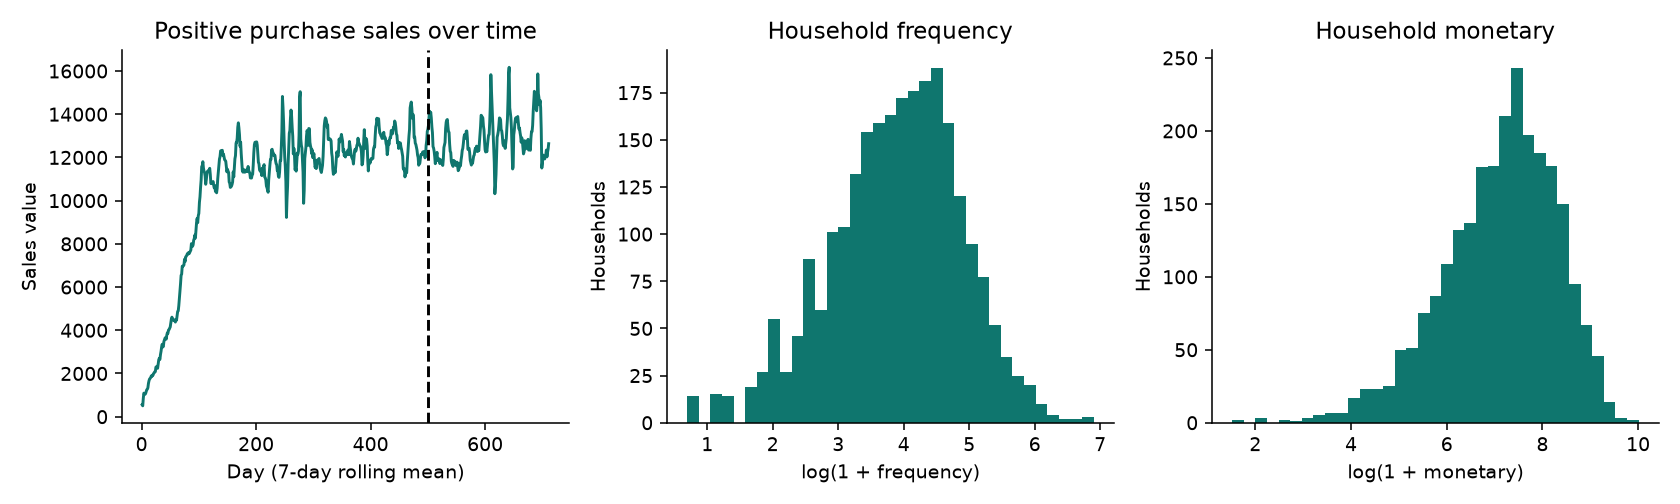
\includegraphics[width=\textwidth]{../figures/01_eda.png}
\caption{Recorded positive-purchase sales and household activity distributions. The dashed temporal boundary marks the calibration/later split on the exact day scale. Household activity is displayed after a log transform because raw purchase intensity is strongly heterogeneous.}\label{fig:eda}
\end{figure}
The EDA motivates a baseline focused on shopping intensity in a transformed distance space. Monetary value and frequency are related because more shopping occasions give more opportunities to spend. Basket-level and assortment measures may repeat the same intensity signal, whereas department shares add preference information directly. The selected eight departments are Grocery, Drug GM, Produce, Meat, Kiosk-Gas, Meat-Packaged, Deli and Pastry.

\section{Model comparisons}
\subsection{Within-space selection}
All three representative K-means models select two clusters under the predeclared minimum-size and silhouette rule. The RFM groups contain 882 and 1,616 households; Behavior contains 809 and 1,689; Product contains 843 and 1,655. These are substantial groups rather than isolated outlier collections.

\begin{table}[htbp]\centering
\caption{Selected K-means models. Silhouette and Davies--Bouldin (DB) values are measured in each model's own space; they do not establish a cross-space ranking.}\label{tab:selected}
\begin{tabular}{lrrrrr}\toprule
Space & Dimensions & $k$ & Smallest group & Silhouette & DB\\\midrule
RFM &3&2&882&0.456&0.857\\
Behavior &8&2&809&0.329&1.237\\
Product &17&2&843&0.206&1.984\\\bottomrule
\end{tabular}\end{table}
\begin{figure}[htbp]\centering
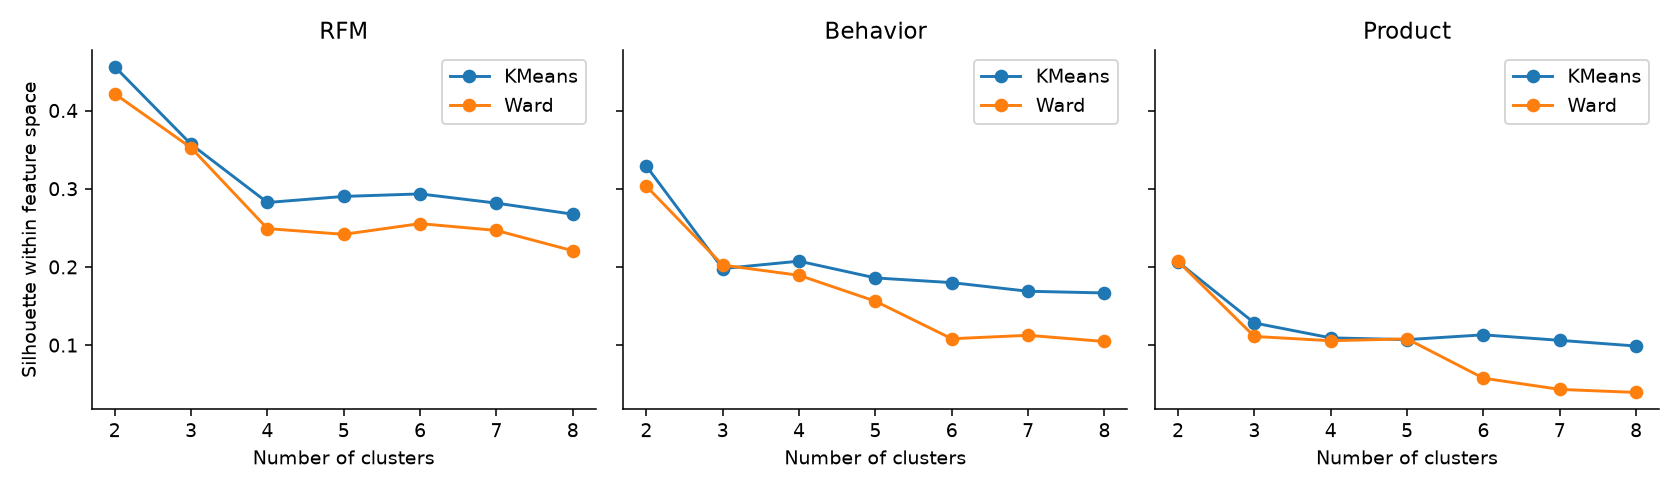
\includegraphics[width=\textwidth]{../figures/02_model_selection.png}
\caption{Candidate K-means and Ward silhouette curves. Compare cluster counts and algorithms within a panel; each panel defines its own distance space.}\label{fig:selection}
\end{figure}
Two groups offer the strongest within-space K-means separation among eligible candidates. Two clusters summarize a continuous intensity gradient rather than two intrinsic household types.

The tested DBSCAN grid does not produce a compelling full-cohort alternative. In RFM at the 70th-percentile neighborhood setting, two groups remain after 18.2\% of households are marked noise, with silhouette 0.162 on retained rows. At tighter settings it yields six groups and negative silhouette. In Behavior, the only two-group setting has a group of just eight households and 14.2\% noise. All tested Product settings produce one non-noise cluster, making multi-cluster silhouette undefined.

\subsection{Stability and partition agreement}
\begin{table}[htbp]\centering\small
\caption{ARI stability. Subsample columns summarize 20 paired independent 80\% samples; reported ranges are empirical minima and maxima, not confidence intervals.}\label{tab:stability}
\begin{tabular}{lrrrr}\toprule
 &\multicolumn{2}{c}{K-means subsamples}&\multicolumn{2}{c}{Ward subsamples}\\
Space & Mean & Range & Mean & Range\\\midrule
RFM &0.980&0.948--1.000&0.535&0.011--0.874\\
Behavior &0.970&0.923--0.995&0.457&0.154--0.740\\
Product &0.964&0.860--0.990&0.314&$-0.024$--0.584\\\bottomrule
\end{tabular}\end{table}
\begin{figure}[htbp]\centering
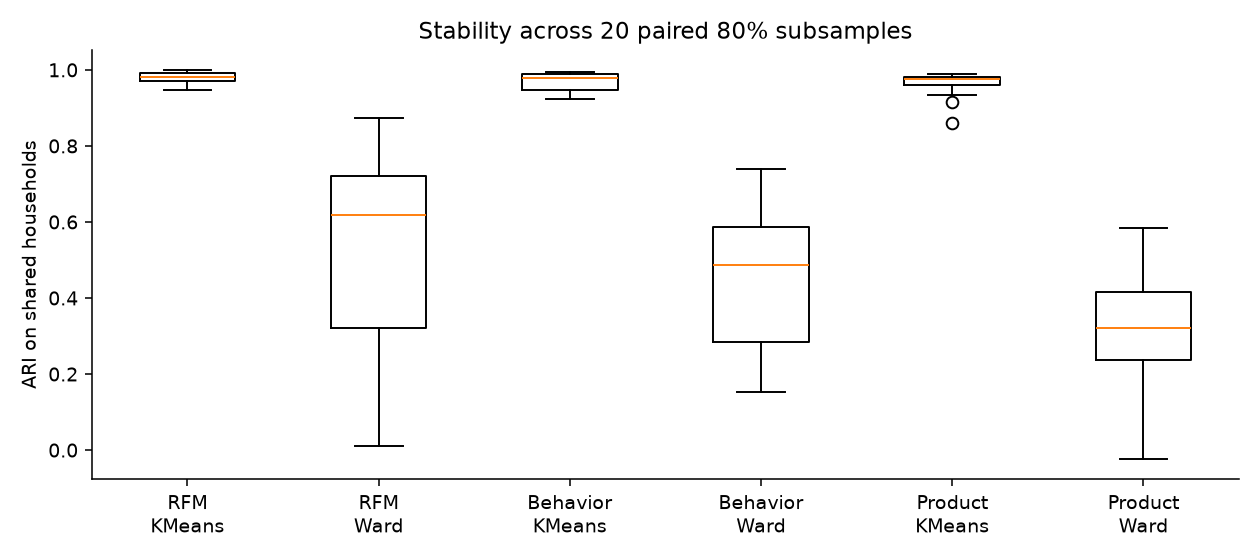
\includegraphics[width=.94\textwidth]{../figures/03_stability.png}
\caption{Conditional sampling stability on shared households. The K-means partitions are substantially more reproducible than Ward under this perturbation.}\label{fig:stability}
\end{figure}
Mean one-initialization ARI against the selected K-means fit is 0.994 for RFM, 0.982 for Behavior and 0.997 for Product. The main findings do not depend on one random start. K-means sampling stability remains high in all three spaces; Product's minimum subsample agreement is lower, so the additional representation does not improve robustness. Ward is substantially more sensitive to household sampling, especially in Product space. K-means is the more reproducible method.

Across selected partitions, RFM--Behavior ARI is 0.614, RFM--Product is 0.589 and Behavior--Product is 0.850. Enrichment changes some assignments, and Product is much closer to Behavior than RFM. Assignment change matters only if it reveals useful new profile distinctions. Numeric cluster identifiers are space-specific; Product cluster 0 corresponds to the higher-activity group, whereas the higher-activity RFM and Behavior group is numbered 1.

\section{Profiles and later-period descriptive checks}
\begin{table}[htbp]\centering\small
\caption{Calibration profiles in original units. Means are descriptive household averages. H and L denote higher- and lower-activity groups within a space, not common fixed memberships.}\label{tab:profiles}
\begin{tabular}{llrrrr}\toprule
Space & Group & $n$ & Recency (days) & Baskets & Recorded sales\\\midrule
RFM &L&882&67.9&20.8&507.7\\
RFM &H&1,616&6.2&104.4&3,034.0\\
Behavior &L&809&68.9&23.8&418.1\\
Behavior &H&1,689&8.4&99.4&2,967.7\\
Product &L&843&65.8&25.5&448.4\\
Product &H&1,655&8.7&100.1&3,004.7\\\bottomrule
\end{tabular}\end{table}
All representations chiefly separate higher-intensity, recently active households from less-frequent and less-recent households. In Product, higher-activity households average 549.7 distinct products and 12.8 departments, versus 114.1 products and 7.6 departments in the lower-activity group. They also have larger mean baskets (35.6 versus 23.0 sales units). Discount-line proportions are close (50.4\% versus 48.9\%), so the two groups are not distinct discount-response types.

\begin{figure}[htbp]\centering
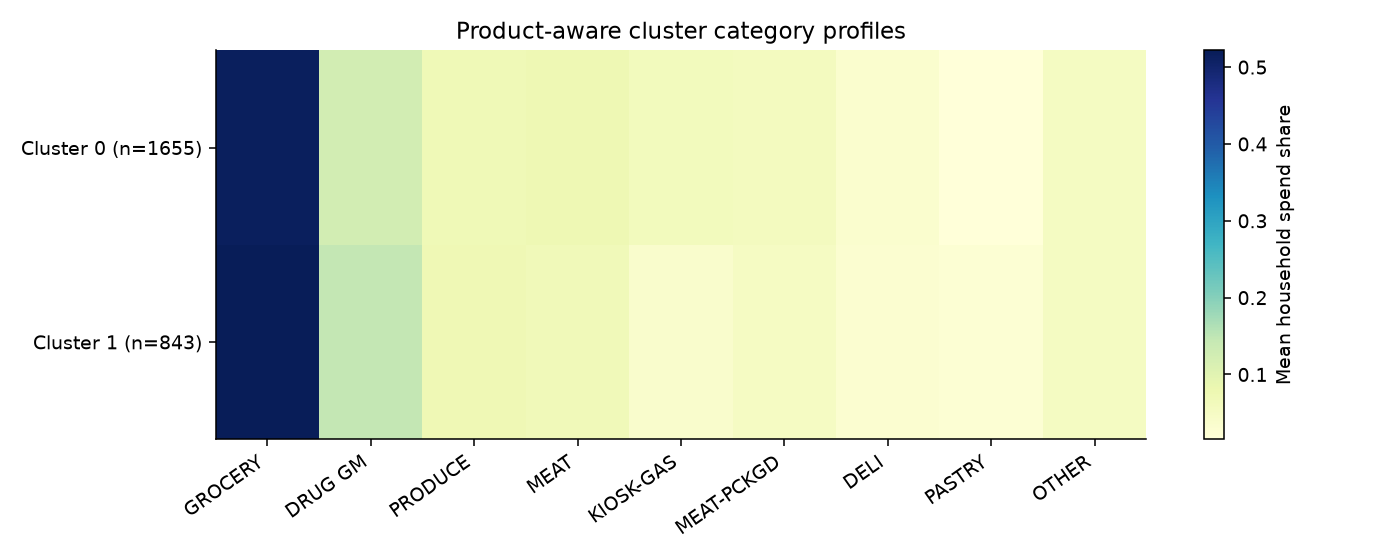
\includegraphics[width=\textwidth]{../figures/04_category_profiles.png}
\caption{Product-aware department profiles: mean of household spend shares, rather than a share of pooled group revenue. Grocery dominates both groups; the modest contrasts qualify how much preference-specific structure the two-group solution reveals.}\label{fig:composition}
\end{figure}
Both Product groups allocate about half of spending to Grocery (51.4\% in the higher-activity group and 52.2\% in the lower). The higher-activity group has a greater Kiosk-Gas share (6.0\% versus 3.7\%) and Meat share (7.5\% versus 6.6\%), while the lower-activity group has more Drug GM (14.5\% versus 12.3\%) and Pastry (2.4\% versus 1.6\%). These differences are useful descriptions but small in absolute terms.

\begin{table}[htbp]\centering\small
\caption{Later-period positive-purchase sales by frozen group. Brackets are 95\% percentile bootstrap intervals for group means, conditional on the fixed clustering; activity is the proportion with any observed later purchase.}\label{tab:later}
\begin{tabular}{llrrr}\toprule
Space & Group & Mean later sales [interval] & Later active & $\eta^2$\\\midrule
RFM &L&343.2 [318.3, 371.2]&93.9\%&0.204\\
RFM &H&1,487.5 [1,424.0, 1,547.0]&99.7\%&\\
Behavior &L&306.3 [280.7, 332.1]&93.7\%&0.197\\
Behavior &H&1,455.7 [1,393.7, 1,516.8]&99.5\%&\\
Product &L&320.8 [297.6, 347.1]&94.1\%&0.202\\
Product &H&1,471.9 [1,413.7, 1,535.6]&99.5\%&\\\bottomrule
\end{tabular}\end{table}
\begin{figure}[htbp]\centering
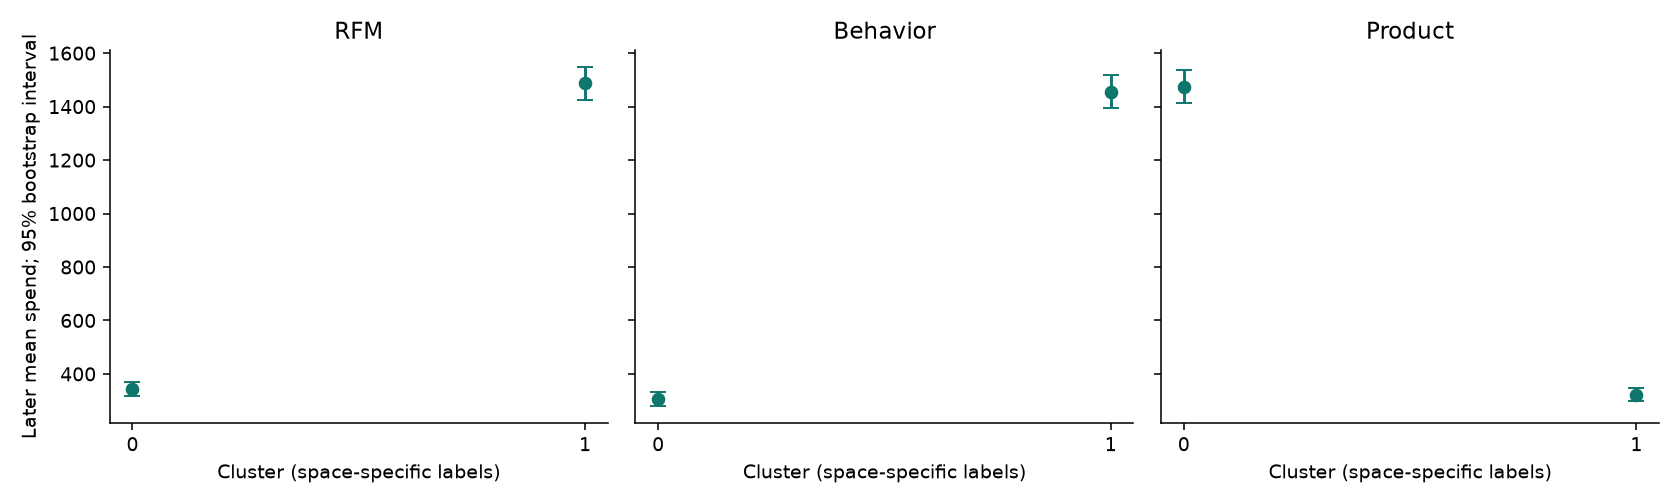
\includegraphics[width=\textwidth]{../figures/05_holdout.png}
\caption{Later mean spending and bootstrap uncertainty. Calibration-defined groups remain descriptively different, with much larger within-cohort purchase intensity in the higher-activity group. Labels are independent in each panel.}\label{fig:holdout}
\end{figure}
The frozen groups retain a large later-period spending difference. Nevertheless, Product explains 20.2\% of later spend variance, compared with 20.4\% for RFM and 19.7\% for Behavior. The absolute Product--RFM difference is approximately $-0.002$ in $\eta^2$. Product therefore brings no improvement on this criterion, and most variance remains within groups.

The intervals reflect group-mean uncertainty, not the uncertainty of a difference between representations. Because the models use the same households, a paired household bootstrap of Product-minus-RFM explained variance gives $-0.00190$, with a conditional 95\% interval $[-0.01426,0.00860]$. This provides no clear evidence of improvement. Holdout results were not used in model selection.



\clearpage
\section{Who changes groups, and why?}\label{sec:cases}
A change in membership is easiest to understand at household level. Cluster numbers themselves cannot be compared across independently fitted models. We first match Product labels to RFM labels by maximum household overlap, then inspect households whose matched assignments differ. From each direction of change, we select the household nearest its transition group's centroid in the transformed Product feature space, breaking distance ties by household identifier. The selection uses calibration data only. The comparison concerns the full enrichment from RFM to Product, including basket behavior; it cannot attribute every change to department preferences alone.

After alignment, 287 of 2,498 households (11.5\%) change groups: 163 move from RFM's lower-activity group to Product's higher-activity group, and 124 move in the reverse direction. These are cross-model reassignments of the same calibration households, not changes over time.

\textbf{Household 2389: broader shopping despite less recent activity.} This household last purchased 33 days before the reference day, made 43 baskets and recorded 1,102.61 in sales. Its 342 products across 13 departments accompany a move from the lower RFM group to the higher Product group. Meat accounts for 12.9\% of spending and Produce 7.8\%. The richer representation incorporates breadth and basket behavior that RFM does not explicitly encode.

\textbf{Household 1970: recent visits with smaller baskets.} With recency of seven days and 44 baskets, this household moves from the higher RFM group to the lower Product group. Recorded sales total 615.01; mean basket sales are 13.98, compared with 25.64 for household 2389. Grocery and Drug GM account for 66.5\% and 17.9\% of spending, with 214 products across eight departments. Similar visit counts therefore need not imply similar basket scale or mix.

Both the basket variables and the department block change between RFM and Product, so these examples do not isolate the effect of one variable.

\begin{figure}[htbp]\centering
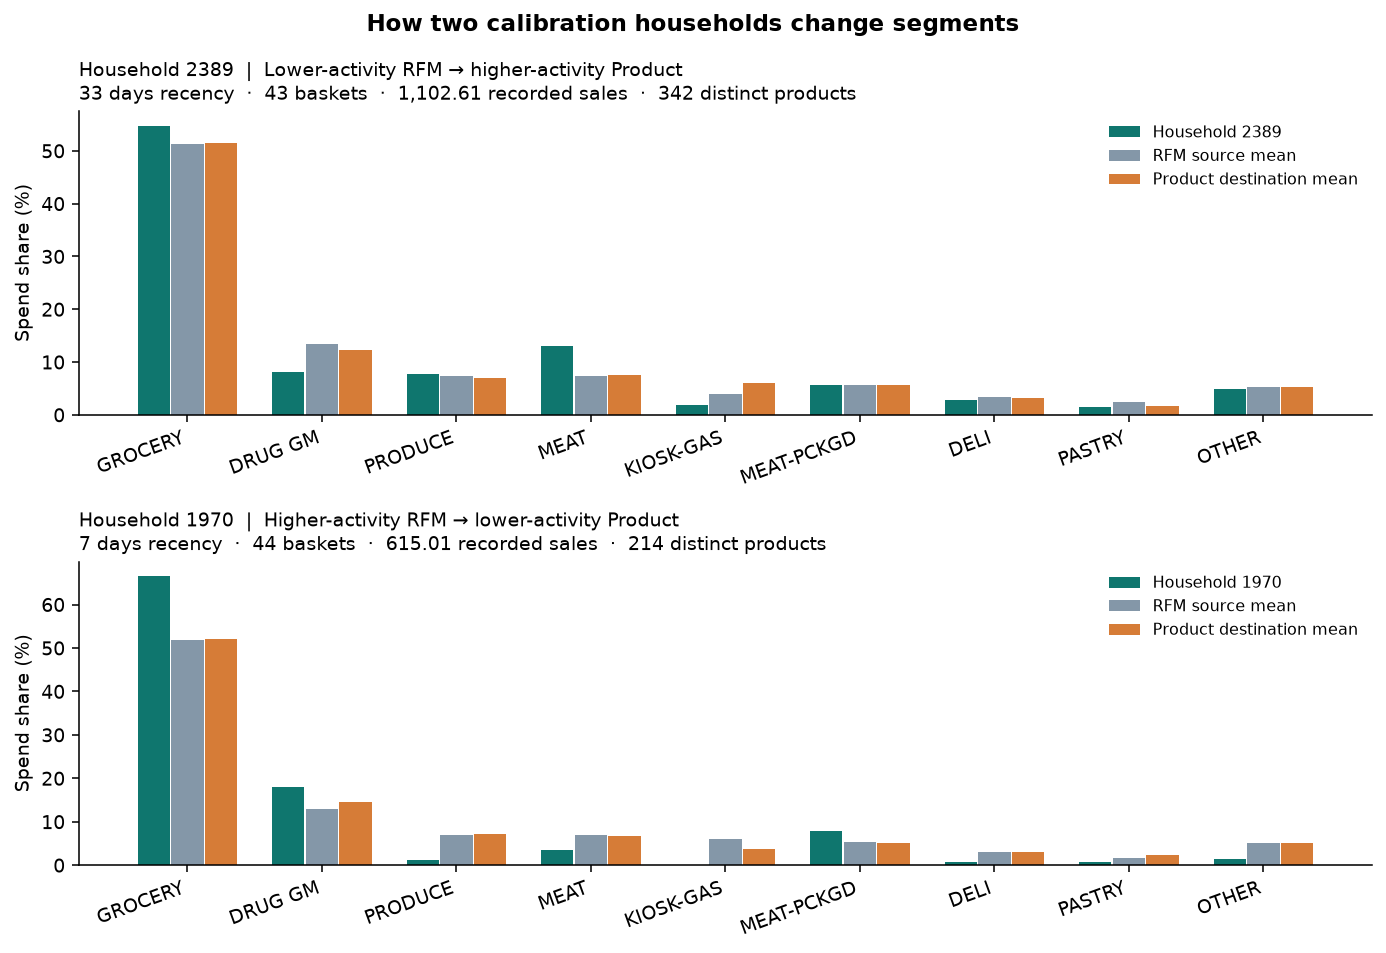
\includegraphics[width=\textwidth]{../figures/10_household_cases.png}
\caption{Actual calibration households selected by a reproducible rule from the changed-membership groups. Sales and basket counts describe the calibration period only. These cases illustrate how different definitions of similarity change a household's assignment.}\label{fig:cases}
\end{figure}

\section{Do department differences persist later?}\label{sec:futurecategories}
The original later-spending criterion is naturally related to RFM's monetary feature. We therefore add a category-specific descriptive check: do the frozen groups distinguish later department spending shares? This extension was designed after the original holdout results had been inspected. It is exploratory and leaves the original feature fitting, cluster-count selection and frozen memberships unchanged.

The category vocabulary remains the eight largest calibration departments plus Other. Later purchases in any department outside that vocabulary enter Other. We calculate each household's department shares separately and give each household equal weight. Shares are undefined for the 59 calibration households with no positive later purchase: they remain in the full-cohort spending and activity results, but the category-composition comparison uses the same 2,439 active households for every representation. This separates absence of purchases from preference for a department.

\begin{figure}[htbp]\centering
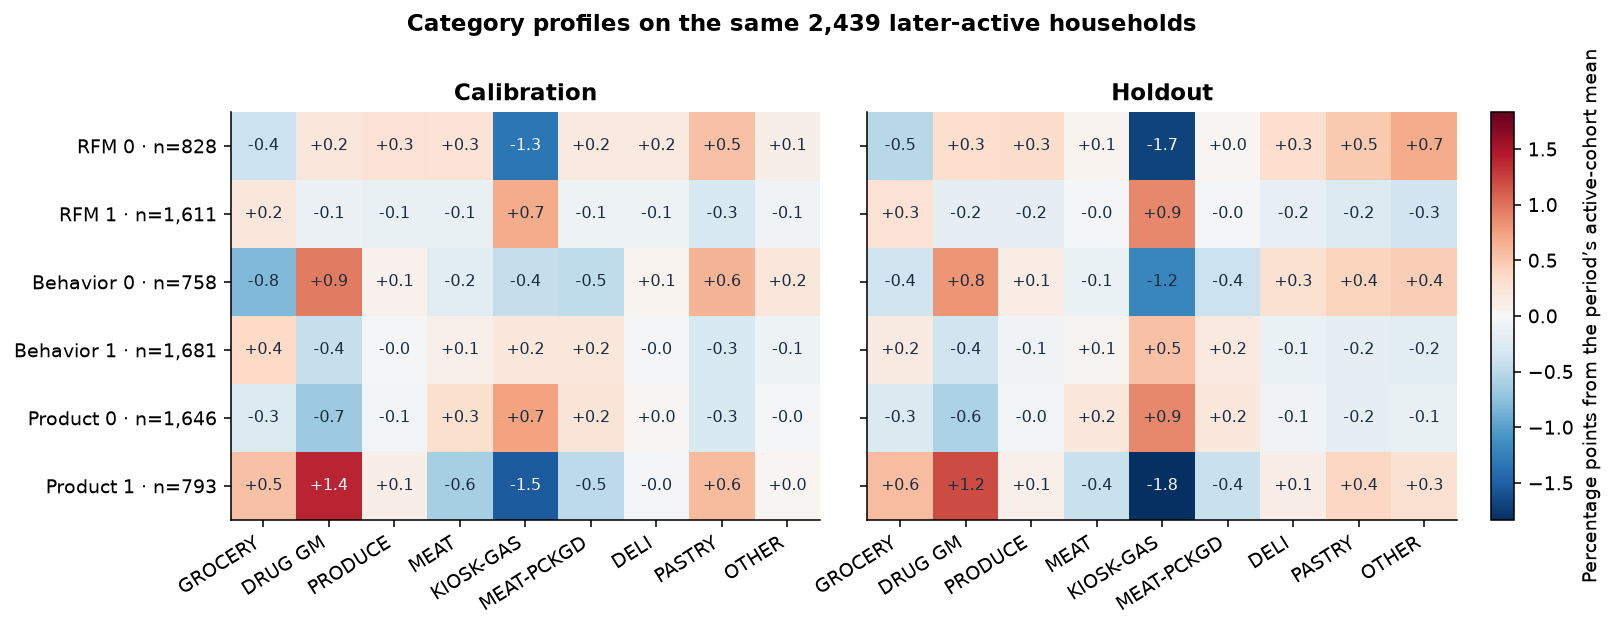
\includegraphics[width=\textwidth]{../figures/12_future_categories.png}
\caption{Department-share deviations for frozen groups. Calibration and later profiles use the same later-active household cohort, with each period centered on that cohort's mean household share. A repeated direction of deviation suggests persistence.}\label{fig:futurecategories}
\end{figure}

For household share vector $\mathbf{s}_i$ and frozen group $g$, the category separation measure is
\[
\eta^2_{\mathrm{category}}=
\frac{\sum_g n_g\lVert\overline{\mathbf{s}}_g-\overline{\mathbf{s}}\rVert^2}
{\sum_i\lVert\mathbf{s}_i-\overline{\mathbf{s}}\rVert^2}.
\]
It is the fraction of total squared variation in nine-component household shares that lies between group means. This raw-share Euclidean summary weights departments by their observed variation. We compare Product minus RFM using 1,000 paired household bootstrap replicates (seed 2027), keeping fitted memberships fixed.

\begin{table}[htbp]\centering
\caption{Exploratory category-share separation on the identical 2,439 later-active households. Entries are percentages of total squared share variation explained by frozen group means, not percentages of shoppers or sales.}\label{tab:categoryholdout}
\begin{tabular}{lrr}\toprule
Representation & Calibration & Later period\\\midrule
RFM & 0.250\% & 0.299\%\\
Behavior & 0.221\% & 0.180\%\\
Product & 0.529\% & 0.386\%\\\bottomrule
\end{tabular}
\end{table}

Product has the largest point estimate for later category separation, but it explains only 0.386\% of the total variation in household shares, versus 0.299\% for RFM. The Product-minus-RFM difference is $0.000868$ on the fraction scale (0.087 percentage points), with a conditional 95\% interval of $[-0.001097,0.003148]$. The interval spans zero, so there is no clear improvement.

Some profile directions do persist. Among the later-active cohort, Product's lower-activity group is 1.39 percentage points above the calibration cohort mean for Drug GM and 1.20 points above the later mean. Its Kiosk-Gas deviations are $-1.53$ and $-1.83$ points respectively. Persistence is not universal: its small Deli deviation changes sign.

\textbf{What this adds to the decision.} Even against department preferences rather than later spending, the two-group Product model shows only a small advantage. Retain RFM for broad activity monitoring and use category profiles as supplementary descriptions.

\section{Fixed-count ablation and sensitivity}
The selected two-group fits already hold cluster count constant. A second paired comparison fixes $k=3$ to ask whether enrichment reveals more useful structure at a moderately finer resolution.
\begin{table}[htbp]\centering\small
\caption{Paired K-means comparison at $k=3$. Common-space silhouette evaluates every assignment in the same standardized RFM coordinates; it tests preservation of RFM geometry, not a neutral measure of all possible usefulness.}\label{tab:fixed}
\begin{tabular}{lrrrr}\toprule
Space & Smallest group & Common RFM silhouette & Mean subsample ARI & Later $\eta^2$\\\midrule
RFM &397&0.357&0.970&0.313\\
Behavior &614&0.138&0.763&0.215\\
Product &677&0.079&0.929&0.170\\\bottomrule
\end{tabular}\end{table}
At three clusters, RFM retains stronger sampling reproducibility than either extension and explains a larger fraction of later-spend variance. Product is more stable than Behavior in this finer partition, but still offers no later-spend separation improvement over RFM. The paired bootstrap Product-minus-RFM difference in later $\eta^2$ is $-0.143$, with a conditional 95\% interval $[-0.165,-0.119]$. This is weaker stratification for the spending criterion. The common-space scores show that the enriched assignments depart from the baseline's geometry, as expected when the definition of similarity changes.

\begin{figure}[htbp]\centering
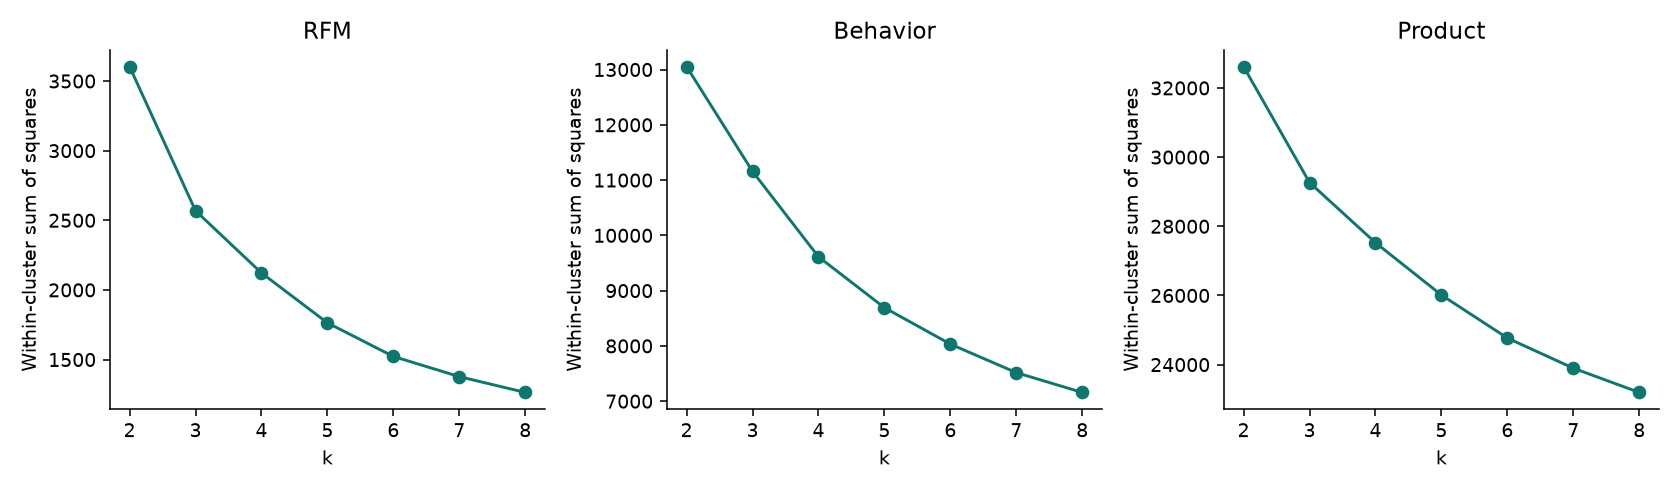
\includegraphics[width=\textwidth]{../figures/07_elbow.png}
\caption{K-means objective over the candidate cluster counts. Read each elbow within its own representation. Absolute inertia values across spaces have different scales and are not a ranking of model quality.}\label{fig:elbow}
\end{figure}
The Product representation's block weight is consequential. At fixed $k=3$, multiplying its category coordinates by 0.5 produces ARI 0.433 against the equal-block model; multiplying them by 2 produces ARI 0.460. Because variance scales with the square of a coordinate multiplier, these settings change the category block's variance to one quarter and four times its default. Such changes lead to materially different memberships even though all use the same data. An optimizer can reproducibly find an answer to a representation choice that remains debatable, so high repeated-start stability does not offset this sensitivity.


\begin{figure}[htbp]\centering
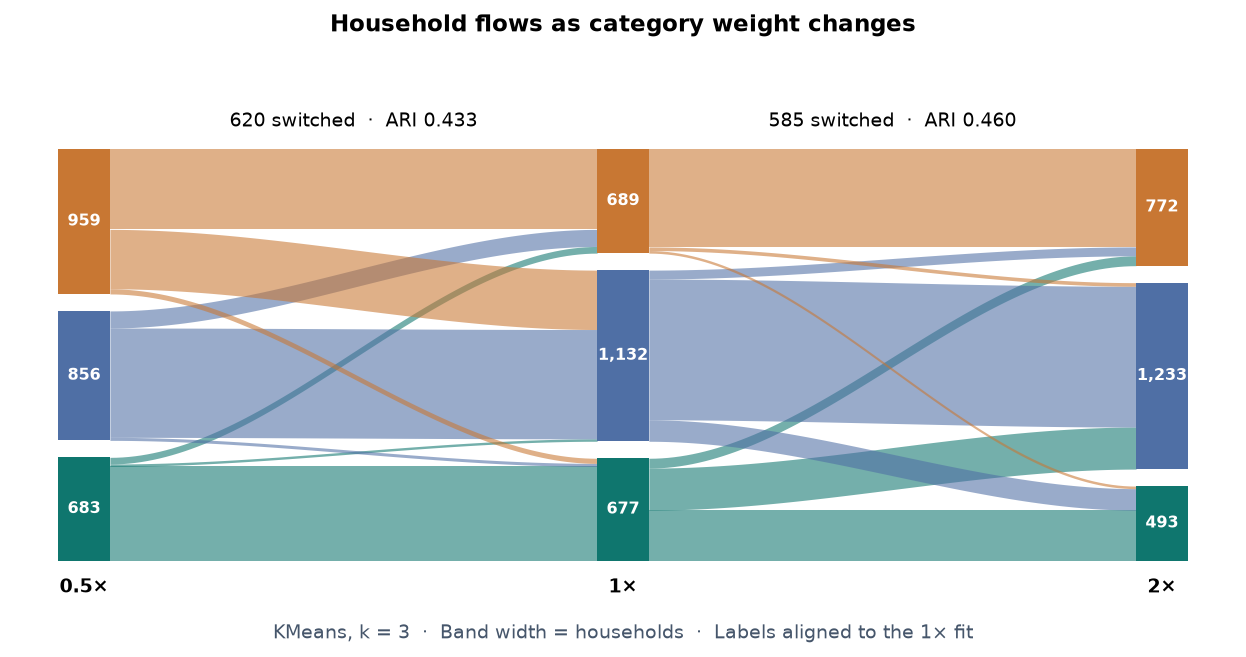
\includegraphics[width=\textwidth]{../figures/11_category_flow.png}
\caption{Household membership at three category-coordinate weights, holding $k=3$ fixed. Ribbon widths count households. Nondefault labels are matched to the default partition by maximum overlap; color is a visual correspondence, not a claim of identical cluster meaning. ARI remains invariant to label numbering.}\label{fig:flow}
\end{figure}
After maximum-overlap label alignment, halving the default category-coordinate weight changes 620 of 2,498 memberships (24.8\%), while doubling it changes 585 (23.4\%).

The flow view separates two questions: whether the optimizer repeatedly finds the same answer at a fixed weight, and whether that answer survives a different definition of similarity. Strong initialization stability answers the first question only. A practical segmentation should disclose the weighting choice and inspect the households affected by it.

\section{Practical interpretation and limitations}
\subsection{What the evidence supports}
RFM K-means with two groups is the best-performing model for this cohort. It is parsimonious, the most reproducible under household resampling (mean subsample ARI 0.980), and at least as informative for later spending separation as the enriched alternatives ($\eta^2=0.204$). The evidence supports two broad activity tiers rather than exactly two consumer types. Product-aware features add interpretable department descriptions and change household membership, but do not improve the principal diagnostics. The later-category check gives a small advantage (0.386\% versus 0.299\% of share variation explained) whose paired difference interval spans zero.

For a retailer, the practical implication is to use the RFM tiers for descriptive monitoring: compare assortment coverage, return activity and basket patterns between higher- and lower-activity households, and look for subgroups with unmet needs. Department profiles can supplement these tiers. Targeting decisions such as which coupon to send or which household to prioritize need an explicit objective and an experiment measuring incremental outcomes.

\subsection{Limitations}
The data are a historical panel from one retailer and do not capture total household grocery demand. Panel enrollment, incomplete observation, seasonality and store assortment may influence behavior, and the results may not generalize to current shoppers or another market. Positive-purchase filtering omits returns and zero-sales lines, so monetary features represent recorded buying activity rather than net margin. No observed later purchase does not prove defection.

Only one temporal split is examined. The 500-day calibration may blur changing preferences, and the 211-day holdout can have a different seasonal mix. Later spend favors historical spending features, so Product-aware groups might matter for a different objective, such as assortment breadth or category demand. All findings are observational and descriptive. The study does not estimate coupon responsiveness, campaign return, margin, customer lifetime value or causal marketing lift, and there is no independent ground truth or external replication.

The candidate grid is limited, DBSCAN tuning is exploratory, and only Euclidean K-means and Ward variants are tested. Correlated behavior features and category block weighting affect distances, and the $k=3$ check shows that weighting materially changes membership. Composition is coarse, with eight departments plus Other. Stability checks and bootstrap intervals condition on fixed preprocessing and fitted groups, and twenty resampling repetitions are a diagnostic rather than a population confidence interval. A PCA projection loses dimensions and is not proof of separability.

\subsection{Future improvements}
A stronger follow-up would predefine the retail decision and a relevance metric independent of feature development, repeat the analysis over rolling temporal origins, and refit the entire pipeline within resampling. It would compare multiple category resolutions and prespecified composition weights, extend the household case studies to systematic transition analysis, and monitor membership drift. A category-specific objective could show whether preference information adds value beyond intensity, and randomized trials would measure targeting benefits and costs.

\section{Conclusion}
\textbf{Main insights.} Adding basket behavior and department preferences to RFM does not improve household segmentation. All representative K-means fits select two broad activity groups, and K-means is more reproducible than Ward. The two groups separate recently active, high-frequency households from infrequent ones. Product features add department descriptions, but membership changes materially with category weighting (287 households change groups between RFM and Product). The exploratory later-category analysis shows some persistent profile differences, but no clear improvement over RFM in overall category-share separation. Coupon records that never entered clustering confirm the split: among households targeted by campaigns starting after day 500, 25.7\% of the RFM higher-activity group redeemed a coupon versus 4.8\% of the lower group, and Product labels do not separate responders better (Section~\ref{sec:extensions}).

\textbf{Best-performing model.} RFM K-means with $k=2$ performs best. It has the highest sampling stability (mean subsample ARI 0.980 versus 0.964 for Product) and the highest later-spend explained variance (0.204 versus 0.202). The fixed three-group comparison also favors RFM. It reaches these results with three features instead of seventeen.

\textbf{Business implications.} Use RFM tiers as the default for broad activity monitoring and treat department profiles as supplementary descriptions. For campaign planning, the four-group RFM persona view (loyal high-value, steady regulars, occasional shoppers and lapsed or at-risk households) re-slices the same activity gradient into actionable tiers: the loyal high-value group is 27.2\% of households but 56.6\% of later spend. A more complex segmentation is justified only for a validated category-specific objective.

\textbf{Limitations.} The data cover one retailer and one temporal split, and the findings are observational: they do not measure campaign lift or causal effects. Demographic data cover almost only higher-activity households, so they cannot profile the lower group.

\textbf{Future improvements.} Predefine the retail decision, repeat the analysis across rolling temporal origins, refit the full pipeline within resampling, test category resolutions and weights, and run randomized trials to measure targeting value.

\bibliographystyle{plain}
\bibliography{references}
\end{document}
